\section{测度的构造}
\label{sec:measure-construction}

上一节规定了测度应满足的规则，并用计数、点质量等例子验证了这些规则可以实现。可是第~\ref{sec:measure-size-additivity}节真正想要的长度测度还没有出现：我们只知道区间的长度，并不知道怎样把它可数可加地推广到$\mathcal B(\mathbb R)$。本节先把第~\ref{sec:measure-jordan}小节中的可数覆盖做成外测度，从中筛选出满足分割可加性的集合；再用这个方法构造实轴上的Lebesgue测度，研究它的逼近性质；然后抽象出从简单集合族延拓测度的存在性与唯一性定理，最后把长度增量换成单调函数的增量，得到Lebesgue--Stieltjes测度。

\subsection{外测度}
\label{sec:measure-outer-measure}

\paragraph{覆盖的总代价}
有理点集的例子提示了一种测量方式：用一列简单集合覆盖待测集合，计算覆盖的总代价，再让总代价尽量小。这个量对每个子集都有定义，它满足的规则比测度少。

\begin{definition}[外测度]
\label{def:measure-outer}
集合$X$上的\term{外测度}（outer measure）是映射$\mu^*:\mathcal P(X)\to[0,+\infty]$，满足：$\mu^*(\varnothing)=0$；$E\subseteq F$蕴含$\mu^*(E)\le\mu^*(F)$；对任意$E_1,E_2,\dots\subseteq X$，$\mu^*(\bigcup_nE_n)\le\sum_n\mu^*(E_n)$。
\end{definition}

\begin{lemma}[由覆盖得到外测度]
\label{lem:measure-cover-outer}
设$\mathcal C$是$X$的一族子集，$\varnothing\in\mathcal C$，$\rho:\mathcal C\to[0,+\infty]$满足$\rho(\varnothing)=0$。对$E\subseteq X$令
\[
 \mu^*(E)=\inf\Bigl\{\sum_{n\ge1}\rho(C_n):C_n\in\mathcal C,\ E\subseteq\bigcup_{n\ge1}C_n\Bigr\},
\]
没有覆盖时取$+\infty$。则$\mu^*$是外测度。
\end{lemma}

\begin{proof}
取全部$C_n=\varnothing$覆盖空集，得$\mu^*(\varnothing)=0$。若$E\subseteq F$，覆盖$F$的每一列集合也覆盖$E$，下确界取在更大的范围上，故$\mu^*(E)\le\mu^*(F)$。对次可加性，不妨设$\sum_n\mu^*(E_n)<+\infty$，任取$\varepsilon>0$。对每个$n$按下确界的定义选覆盖$E_n$的$C_{n,1},C_{n,2},\dots\in\mathcal C$，使$\sum_k\rho(C_{n,k})\le\mu^*(E_n)+\varepsilon2^{-n}$。全体$C_{n,k}$可排成一列并覆盖$\bigcup_nE_n$，于是
\[
 \mu^*\Bigl(\bigcup_nE_n\Bigr)\le\sum_n\sum_k\rho(C_{n,k})\le\sum_n\bigl(\mu^*(E_n)+\varepsilon2^{-n}\bigr)=\sum_n\mu^*(E_n)+\varepsilon.
\]
非负项的排列不改变级数和，所以这里的双重求和与排成一列后的求和相等。令$\varepsilon\to0$即得结论。
\end{proof}

外测度能给每个子集赋值，代价是失去可加性。在$X=\{1,2\}$上取$\mathcal C=\{\varnothing,X\}$、$\rho(X)=1$，则唯一的有效覆盖是$X$本身，$\mu^*(\{1\})=\mu^*(\{2\})=\mu^*(X)=1$。不交的$\{1\}$与$\{2\}$外测度之和为$2$，并的外测度却是$1$。原因是覆盖无法把两点分开计价，只能整体付费。因此外测度一般不是$\mathcal P(X)$上的测度，需要找出它在哪些集合上可加。

\paragraph{Carathéodory可测性}
设想用集合$A$把任一测试集合$E$切成$E\cap A$与$E\setminus A$两部分。若对一切$E$，两部分外测度之和都等于$\mu^*(E)$，就说明$A$的边界不会让覆盖“多付费”，可以把$A$当作可测集合。

\begin{definition}[Carathéodory可测]
\label{def:measure-caratheodory-measurable}
设$\mu^*$是$X$上的外测度。若对每个$E\subseteq X$都有
\[
 \mu^*(E)=\mu^*(E\cap A)+\mu^*(E\setminus A),
\]
称$A\subseteq X$为$\mu^*$-\term{Carathéodory可测}（Carathéodory measurable）的。
\end{definition}

由次可加性，“$\le$”总是成立，所以验证时只需证明“$\ge$”，并且只需对$\mu^*(E)<+\infty$的$E$验证。上例中$\{1\}$不满足判据：取$E=X$，右边为$2$，左边为$1$。

\begin{theorem}[Carathéodory定理]
\label{thm:measure-caratheodory-criterion}
设$\mu^*$是$X$上的外测度，$\mathcal M$为全体$\mu^*$-Carathéodory可测集。则$\mathcal M$是$\sigma$代数，$\mu^*$在$\mathcal M$上的限制是测度，且$(X,\mathcal M,\mu^*|_{\mathcal M})$完备；特别地，$\mu^*(N)=0$的集合$N$都属于$\mathcal M$。
\end{theorem}

证明分三步：先处理补集与有限并，再控制可数不交并，最后由不交化得到一般可数并，同时读出可数可加性。

\begin{proof}
\emph{补集与有限并。}判据关于$A$与$X\setminus A$对称，所以$\mathcal M$对补集封闭；$X\in\mathcal M$是因为$\mu^*(\varnothing)=0$。设$A,B\in\mathcal M$，$E\subseteq X$。先用$A$切$E$，再用$B$切$E\setminus A$：
\[
 \mu^*(E)=\mu^*(E\cap A)+\mu^*\bigl((E\setminus A)\cap B\bigr)+\mu^*\bigl(E\setminus(A\cup B)\bigr).
\]
由于$E\cap(A\cup B)=(E\cap A)\cup((E\setminus A)\cap B)$，前两项之和不小于$\mu^*(E\cap(A\cup B))$，从而$\mu^*(E)\ge\mu^*(E\cap(A\cup B))+\mu^*(E\setminus(A\cup B))$，即$A\cup B\in\mathcal M$。于是$\mathcal M$对有限并、有限交与差都封闭。

\emph{可数不交并。}设$A_1,A_2,\dots\in\mathcal M$两两不交，$B_n=\bigcup_{k\le n}A_k$，$B=\bigcup_kA_k$。先对$n$归纳证明$\mu^*(E\cap B_n)=\sum_{k\le n}\mu^*(E\cap A_k)$：用$A_n$切测试集合$E\cap B_n$，因$A_n$与$B_{n-1}$不交，得
\[
 \mu^*(E\cap B_n)=\mu^*(E\cap A_n)+\mu^*(E\cap B_{n-1}).
\]
再用$B_n\in\mathcal M$切$E$，并由$E\setminus B_n\supseteq E\setminus B$及单调性，
\[
 \mu^*(E)=\mu^*(E\cap B_n)+\mu^*(E\setminus B_n)\ge\sum_{k\le n}\mu^*(E\cap A_k)+\mu^*(E\setminus B).
\]
令$n\to\infty$，再用次可加性，
\begin{equation}
 \mu^*(E)\ge\sum_{k\ge1}\mu^*(E\cap A_k)+\mu^*(E\setminus B)\ge\mu^*(E\cap B)+\mu^*(E\setminus B).
 \label{eq:measure-caratheodory-chain}
\end{equation}
所以$B\in\mathcal M$。在式~\eqref{eq:measure-caratheodory-chain}中取$E=B$，得$\mu^*(B)\ge\sum_k\mu^*(A_k)$，与次可加性合起来就是$\mu^*(B)=\sum_k\mu^*(A_k)$。

\emph{一般可数并与零外测度集。}对任意$A_n\in\mathcal M$，令$A'_n=A_n\setminus\bigcup_{k<n}A_k$，它们属于$\mathcal M$且两两不交，$\bigcup_nA'_n=\bigcup_nA_n$，由上一步知后者属于$\mathcal M$。因此$\mathcal M$是$\sigma$代数，$\mu^*$在其上可数可加，是测度。若$\mu^*(N)=0$，则对任意$E$，$\mu^*(E\cap N)+\mu^*(E\setminus N)\le0+\mu^*(E)$，故$N\in\mathcal M$。零测集的子集外测度也为零，所以属于$\mathcal M$，测度空间完备。
\end{proof}

这个定理只告诉我们$\mathcal M$是$\sigma$代数，并没有保证它含有我们关心的集合；在上面两点的例子中，$\mathcal M=\{\varnothing,X\}$。对具体的外测度，还需要验证想要测量的集合（例如区间）满足判据，这正是下一小节对长度所做的事。

\subsection{Lebesgue测度}
\label{sec:measure-lebesgue}

\paragraph{区间覆盖与Lebesgue外测度}
在引理~\ref{lem:measure-cover-outer}中取$\mathcal C$为全体开区间（连同空集），$\rho$为长度，得到实轴上的外测度
\[
 \lambda^*(E)=\inf\Bigl\{\sum_{n\ge1}(b_n-a_n):E\subseteq\bigcup_{n\ge1}(a_n,b_n)\Bigr\},\qquad E\subseteq\mathbb R,
\]
称为\term{Lebesgue外测度}（Lebesgue outer measure）。由引理~\ref{lem:measure-cover-outer}，它满足空集为零、单调性与可数次可加性。图~\ref{fig:measure-outer-cover}示意了它的计算：覆盖可以重叠，也可以用越来越短的区间处理零散的点，下确界衡量的是“最节省”的覆盖。要使它成为长度的推广，还需检查两件事：区间的外测度等于长度，以及区间满足Carathéodory判据。

\begin{figure}[!htbp]
  \centering
  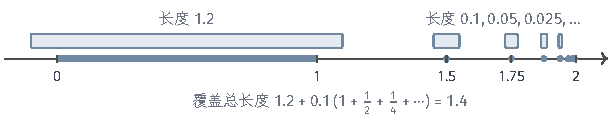
\includegraphics[width=103.7mm]{figures/02-abstract-mathematics/01-metric-and-measure/tikz/c2-outer-cover/figure.pdf}
  \caption{用可数个开区间覆盖集合$E=[0,1]\cup\{1.5,1.75,1.875,\dots\}$（深色）。浅色区间是一种覆盖：区间$(-0.1,1.1)$覆盖线段部分，长度依次减半的小区间覆盖离散的点。覆盖总长度为$1.2+0.1\cdot(1+\tfrac12+\tfrac14+\cdots)=1.4$；把各区间进一步缩短，总长度可以任意接近$1$，因此$\lambda^*(E)=1$。}
  \label{fig:measure-outer-cover}
\end{figure}

\paragraph{区间的外测度}
下界的困难在于覆盖可以有无限多个区间。闭区间的紧性把它化为有限覆盖，而有限覆盖可以沿实轴从左到右逐个检查。为了在第~\ref{sec:measure-stieltjes}小节复用，下面把长度换成单调函数的增量来叙述，取$F(x)=x$就回到长度。

\begin{lemma}[闭区间的有限开覆盖]
\label{lem:measure-finite-cover}
设$F:\mathbb R\to\mathbb R$单调不减，$a\le b$，开区间$(c_1,d_1),\dots,(c_m,d_m)$覆盖$[a,b]$。则
\[
 F(b)-F(a)\le\sum_{k=1}^m\bigl(F(d_k)-F(c_k)\bigr).
\]
\end{lemma}

\begin{proof}
对区间个数$m$归纳，同时对一切$a\le b$断言成立。点$b$落在某个区间中，不妨设$c_m<b<d_m$。若$c_m<a$，则$[a,b]\subseteq(c_m,d_m)$，由单调性$F(b)-F(a)\le F(d_m)-F(c_m)$，右边其余各项非负，结论成立。若$c_m\ge a$，则$[a,c_m]$中的点都不在$(c_m,d_m)$中，只能被其余$m-1$个区间覆盖；当$m=1$时这不可能，当$m\ge2$时由归纳假设，$F(c_m)-F(a)\le\sum_{k<m}(F(d_k)-F(c_k))$。再加上$F(d_m)-F(c_m)\ge F(b)-F(c_m)$，两式相加即得。
\end{proof}

\begin{lemma}[区间的Lebesgue外测度]
\label{lem:measure-interval-outer}
对任意区间$I$，$\lambda^*(I)=\ell(I)$；无界区间两边都为$+\infty$。
\end{lemma}

\begin{proof}
先看闭区间$[a,b]$。对任意$\varepsilon>0$，单个区间$(a-\varepsilon,b+\varepsilon)$覆盖它，所以$\lambda^*([a,b])\le b-a+2\varepsilon$。反过来，设开区间$(a_n,b_n)$覆盖$[a,b]$。有界闭区间是紧集（第~\ref{sec:metric-compactness}节的Heine--Borel判据），所以其中有限个，例如$n\le m$的那些，已经覆盖$[a,b]$。由引理~\ref{lem:measure-finite-cover}（取$F(x)=x$），$b-a\le\sum_{n\le m}(b_n-a_n)\le\sum_n(b_n-a_n)$。对一切覆盖取下确界，得$\lambda^*([a,b])\ge b-a$。

对端点为$a<b$的有界区间$I$，任取$0<\varepsilon<(b-a)/2$，有$[a+\varepsilon,b-\varepsilon]\subseteq I\subseteq[a,b]$，由单调性$b-a-2\varepsilon\le\lambda^*(I)\le b-a$，令$\varepsilon\to0$。无界区间包含任意长的闭区间，外测度为$+\infty$。
\end{proof}

\paragraph{区间满足Carathéodory判据}
只需对半直线验证，因为由定理~\ref{thm:measure-borel-generators}，它们生成$\mathcal B(\mathbb R)$。

\begin{lemma}[半直线的可测性]
\label{lem:measure-halfline-measurable}
对每个$a\in\mathbb R$，半直线$H=(a,+\infty)$是$\lambda^*$-Carathéodory可测的。
\end{lemma}

\begin{proof}
设$E\subseteq\mathbb R$，$\lambda^*(E)<+\infty$，任取$\varepsilon>0$，选开区间$I_n$覆盖$E$且$\sum_n\ell(I_n)\le\lambda^*(E)+\varepsilon$。每个$I_n$被点$a$分成两个区间$I_n\cap H$与$I_n\setminus H$（可能为空），长度之和等于$\ell(I_n)$。前者覆盖$E\cap H$，后者覆盖$E\setminus H$，由次可加性和引理~\ref{lem:measure-interval-outer}，
\[
 \begin{aligned}
  \lambda^*(E\cap H)+\lambda^*(E\setminus H)
  &\le\sum_n\ell(I_n\cap H)+\sum_n\ell(I_n\setminus H)\\
  &=\sum_n\ell(I_n)\le\lambda^*(E)+\varepsilon.
 \end{aligned}
\]
令$\varepsilon\to0$即得判据中的“$\ge$”。
\end{proof}

由Carathéodory定理，$\lambda^*$-可测集构成一个$\sigma$代数；它含全部半直线，从而含它们生成的$\mathcal B(\mathbb R)$。

\begin{definition}[Lebesgue测度]
\label{def:measure-lebesgue}
关于$\lambda^*$为Carathéodory可测的全体集合称为\term{Lebesgue可测集}（Lebesgue measurable set），记作$\mathcal L$；$\lambda^*$在$\mathcal L$上的限制$\lambda$称为实轴上的\term{Lebesgue测度}（Lebesgue measure）。$\lambda$在$\mathcal B(\mathbb R)$上的限制也称为Borel集上的Lebesgue测度，仍记作$\lambda$。
\end{definition}

综合以上结果，$(\mathbb R,\mathcal L,\lambda)$是完备测度空间，$\mathcal B(\mathbb R)\subseteq\mathcal L$，并且每个区间的Lebesgue测度等于它的长度。由于覆盖平移后仍是覆盖、长度不变，$\lambda^*(E+t)=\lambda^*(E)$对一切$t\in\mathbb R$成立，Lebesgue测度还具有平移不变性。

\paragraph{可数集的测度}
单点$\{x\}$被$(x-\varepsilon,x+\varepsilon)$覆盖，$\lambda(\{x\})\le2\varepsilon$，故为$0$。由可数次可加性，可数集的Lebesgue测度为$0$。回到第~\ref{sec:measure-jordan}小节的有理点集：$\lambda(\mathbb Q\cap[0,1])=0$，而$[0,1]$中的无理数集合测度为$\lambda([0,1])-0=1$。Jordan外测量把有理点算作$1$，是因为它只允许有限覆盖；可数覆盖把稠密而可数的集合正确地算作零。同时，$[0,1]$是不可数个单点之并，各单点测度为$0$，整体测度却为$1$，这兑现了第~\ref{sec:measure-null-sets}小节的说法：零测集的可数并仍是零测集，不可数并则不然。

\paragraph{Cantor集}
零测集是否一定可数？Cantor集给出否定的回答。

\begin{example}[Cantor集]
\label{ex:measure-cantor-set}
令$C_0=[0,1]$。把$C_{n-1}$中每个闭区间三等分，删去中间的开区间，得到$C_n$，它由$2^n$个长度为$3^{-n}$的闭区间组成，例如$C_1=[0,\tfrac13]\cup[\tfrac23,1]$，$C_2=[0,\tfrac19]\cup[\tfrac29,\tfrac13]\cup[\tfrac23,\tfrac79]\cup[\tfrac89,1]$。令$C=\bigcap_{n\ge0}C_n$，称为\term{Cantor集}（Cantor set）。它是闭集的交，是闭集，因而是Borel集。由$C\subseteq C_n$与有限可加性，
\[
 \lambda(C)\le\lambda(C_n)=2^n\cdot3^{-n}=(2/3)^n\to0,
\]
所以$\lambda(C)=0$。图~\ref{fig:measure-cantor-set}画出了前四步。
\end{example}

\begin{figure}[!htbp]
  \centering
  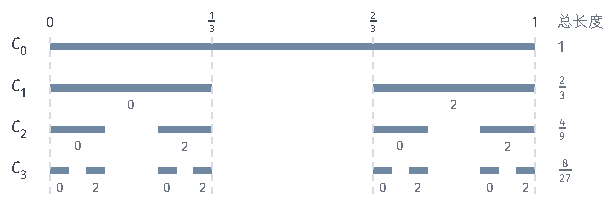
\includegraphics[width=104.1mm]{figures/02-abstract-mathematics/01-metric-and-measure/tikz/c2-cantor-set/figure.pdf}
  \caption{Cantor集构造的前四步。第$n$行$C_n$由$2^n$个长度为$3^{-n}$的闭区间组成，总长度$(2/3)^n$依次为$1,\tfrac23,\tfrac49,\tfrac{8}{27}$；区间下方的三进制数字$0$或$2$记录每一步选择左段还是右段。}
  \label{fig:measure-cantor-set}
\end{figure}

Cantor集虽然测度为零，却不可数。对每个$0$--$1$序列$s=(s_1,s_2,\dots)$，令$\phi(s)=\sum_{k\ge1}2s_k3^{-k}$，即三进制展开中只用数字$0$与$2$的数。按图~\ref{fig:measure-cantor-set}的读法，前$n$位数字决定了在每一步选左段（数字$0$）还是右段（数字$2$），对$n$归纳可知$\phi(s)$落在$C_n$的相应区间中，所以$\phi(s)\in C$。$\phi$是单射：若$s\ne t$且第一个不同的位置为$k$，不妨$s_k=1$、$t_k=0$，则
\[
 \phi(s)-\phi(t)\ge2\cdot3^{-k}-\sum_{j>k}2\cdot3^{-j}=2\cdot3^{-k}-3^{-k}=3^{-k}>0.
\]
全体$0$--$1$序列由对角线方法不可数，因此$C$不可数。可数集测度为零，但测度为零的集合不必可数；零测性度量的是集合占据的长度，基数度量的是元素的多少，二者不能互相推出。

\subsection{Lebesgue测度的逼近与推广}
\label{sec:measure-lebesgue-approximation}

\paragraph{开集外逼近与紧集内逼近}
Lebesgue测度是用开区间覆盖定义的，因此一个可测集合应当能被开集从外面逼近。取补集后，从里面也能用闭集乃至紧集逼近。这一性质把任意可测集合的测量问题化为开集和紧集这两类较好的集合，后面构造连续函数逼近和研究变量替换时都会用到。

\begin{theorem}[Lebesgue测度的正则性]
\label{thm:measure-lebesgue-regularity}
设$E\in\mathcal L$，$\varepsilon>0$。
\begin{enumerate}
 \item 存在开集$U\supseteq E$，使$\lambda(U\setminus E)<\varepsilon$。
 \item 存在闭集$F\subseteq E$，使$\lambda(E\setminus F)<\varepsilon$。
 \item 若$\lambda(E)<+\infty$，存在紧集$K\subseteq E$，使$\lambda(E\setminus K)<\varepsilon$。
\end{enumerate}
\end{theorem}

\begin{proof}
先对$\lambda(E)<+\infty$证明第1条。按$\lambda^*$的定义，存在开区间$I_n$覆盖$E$且$\sum_n\ell(I_n)<\lambda(E)+\varepsilon$。令$U=\bigcup_nI_n$，它是开集，$\lambda(U)\le\sum_n\ell(I_n)<\lambda(E)+\varepsilon$。由于$\lambda(E)$有限，$\lambda(U\setminus E)=\lambda(U)-\lambda(E)<\varepsilon$。一般情形把$E$切成有限测度的片$E_k=E\cap\{x:k-1\le|x|<k\}$，$k\ge1$，对每片取开集$U_k\supseteq E_k$使$\lambda(U_k\setminus E_k)<\varepsilon2^{-k}$；$U=\bigcup_kU_k$是开集，$U\setminus E\subseteq\bigcup_k(U_k\setminus E_k)$，故$\lambda(U\setminus E)<\varepsilon$。

对第2条，把第1条用于补集$\mathbb R\setminus E$，得开集$V\supseteq\mathbb R\setminus E$，$\lambda(V\setminus(\mathbb R\setminus E))<\varepsilon$。令$F=\mathbb R\setminus V$，它是闭集且$F\subseteq E$，而$E\setminus F=E\cap V=V\setminus(\mathbb R\setminus E)$，测度小于$\varepsilon$。

对第3条，先由第2条取闭集$F\subseteq E$使$\lambda(E\setminus F)<\varepsilon/2$。令$K_n=F\cap[-n,n]$，它有界闭，由Heine--Borel判据是紧集。集合$E\setminus K_n$递减，交为$E\setminus F$，且$\lambda(E\setminus K_1)\le\lambda(E)<+\infty$，由从上连续性$\lambda(E\setminus K_n)\to\lambda(E\setminus F)<\varepsilon/2$，所以$n$充分大时$K=K_n$满足要求。
\end{proof}

图~\ref{fig:measure-inner-outer-approx}以$E=[0,1]\setminus\{1/2\}$与$\varepsilon=0.25$为例：外侧开集$U=(-0.05,1.05)$包含$E$且多出的部分长度为$0.1$；内侧紧集$K=[0.05,0.45]\cup[0.55,0.95]$含于$E$，缺少的部分由四段长$0.05$的区间组成，总长度为$0.2$。两者都小于$\varepsilon$。这里逼近的是测度，而不是形状：$U\setminus E$与$E\setminus K$可以由多段组成，只要总长度小。

\begin{figure}[!htbp]
  \centering
  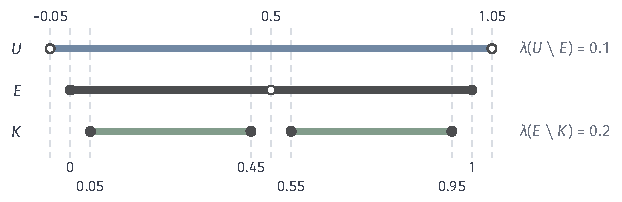
\includegraphics[width=105.3mm]{figures/02-abstract-mathematics/01-metric-and-measure/tikz/c2-inner-outer-approx/figure.pdf}
  \caption{可测集合$E=[0,1]\setminus\{1/2\}$的外开内紧逼近。中行是$E$，空心点表示被去掉的$1/2$；上行开集$U=(-0.05,1.05)\supseteq E$，$\lambda(U\setminus E)=0.1$；下行紧集$K=[0.05,0.45]\cup[0.55,0.95]\subseteq E$，$\lambda(E\setminus K)=0.2$。}
  \label{fig:measure-inner-outer-approx}
\end{figure}

\paragraph{Lebesgue可测集与Borel集}
正则性还说明，Lebesgue可测集与Borel集只差零测集。可数个开集的交是Borel集；对$E\in\mathcal L$，按第1条取开集$U_n\supseteq E$使$\lambda(U_n\setminus E)<1/n$，令$G=\bigcap_nU_n$，则$G\supseteq E$是Borel集，并且$\lambda(G\setminus E)\le\lambda(U_n\setminus E)<1/n$对一切$n$成立，故$\lambda(G\setminus E)=0$。

\begin{theorem}[Lebesgue测度是Borel测度的完备化]
\label{thm:measure-lebesgue-completion}
测度空间$(\mathbb R,\mathcal L,\lambda)$是Borel测度空间$(\mathbb R,\mathcal B(\mathbb R),\lambda)$的完备化：$E\in\mathcal L$当且仅当$E=B\cup M$，其中$B\in\mathcal B(\mathbb R)$，$M$包含于某个Borel零测集，并且此时$\lambda(E)=\lambda(B)$。
\end{theorem}

\begin{proof}
设$E\in\mathcal L$。由上一段，存在Borel集$G\supseteq E$，$\lambda(G\setminus E)=0$。对$\mathcal L$中的零测集$G\setminus E$再用一次上一段的结论，得Borel集$G'\supseteq G\setminus E$，$\lambda(G')=0$。于是$E=(G\setminus G')\cup(E\cap G')$，第一项是Borel集，第二项包含于Borel零测集$G'$，且$\lambda(E)=\lambda(G\setminus G')$。反过来，$\mathcal L$包含$\mathcal B(\mathbb R)$并且完备（定理~\ref{thm:measure-caratheodory-criterion}），所以每个$B\cup M$都属于$\mathcal L$，测度为$\lambda(B)$。
\end{proof}

由此可以区分三个范围：$\mathcal B(\mathbb R)\subseteq\mathcal L\subseteq\mathcal P(\mathbb R)$。两个包含都是严格的。Cantor集$C$测度为零，由完备性它的全部子集都Lebesgue可测，这样的子集比Borel集多，所以存在不是Borel集的Lebesgue可测集；这里的基数比较需要说明Borel集全体与$\mathbb R$等势，本章不展开。另一方面，借助选择公理可以构造不Lebesgue可测的集合（Vitali构造），我们只把它作为边界记住：并非所有子集都能被赋予与长度相容的测度，这正是测度只定义在$\sigma$代数上的原因。日常使用中，Borel集已经足够；需要“零测集的子集可测”时，再换用完备化。

\paragraph{多维Lebesgue测度}
在$\mathbb R^d$上，把区间换成开矩形$R=\prod_{i=1}^d(a_i,b_i)$（各边与坐标轴平行），长度换成体积$\prod_{i=1}^d(b_i-a_i)$，用可数个开矩形覆盖并对总体积取下确界，就得到外测度$\lambda_d^*$。上面的步骤逐一对应：闭矩形紧致，把可数覆盖化为有限覆盖后，用全部矩形的边坐标把一个大矩形切成网格，比较各网格小块的体积，可得闭矩形的外测度等于体积；把每个覆盖矩形沿超平面$\{\bm x:x_i=a\}$切成两个矩形，可得半空间$\{\bm x:x_i>a\}$满足Carathéodory判据；开集是可数个有理顶点开矩形之并，所以半空间生成$\mathcal B(\mathbb R^d)$。由此得到$\mathcal B(\mathbb R^d)$上体积的推广$\lambda_d$，称为$d$维Lebesgue测度，正则性与完备化的论证不变。$\lambda_d$与$d$个实轴Lebesgue测度的乘积在Borel集上相同，这一点需要乘积测度与唯一性定理，在第~\ref{sec:integral-iterated}节证明，那里也将区分乘积$\sigma$代数与其完备化。

\subsection{测度延拓的存在性和唯一性}
\label{sec:measure-extension}

\paragraph{从预测度延拓}
Lebesgue测度的构造可以抽象出来：先在一族简单集合上给出可数可加的赋值，再用覆盖得到外测度，最后由Carathéodory定理得到$\sigma$代数上的测度。这族简单集合只需对有限运算封闭。

\begin{definition}[集合代数与预测度]
\label{def:measure-algebra-premeasure}
$X$的一族子集$\mathcal R$若含$X$，并对补集和有限并封闭，称为$X$上的\term{集合代数}（algebra of sets）。$\mathcal R$上的映射$\mu_0:\mathcal R\to[0,+\infty]$若满足$\mu_0(\varnothing)=0$，并且对两两不交、并集仍属于$\mathcal R$的$A_1,A_2,\dots\in\mathcal R$有$\mu_0(\bigcup_nA_n)=\sum_n\mu_0(A_n)$，称为$\mathcal R$上的\term{预测度}（premeasure）。若存在$X_n\in\mathcal R$使$X=\bigcup_nX_n$且$\mu_0(X_n)<+\infty$，称$\mu_0$是$\sigma$有限的。
\end{definition}

集合代数只保证有限运算的结果仍在其中，可数并可能跑出去，所以预测度的可数可加性只在并集仍属于$\mathcal R$时提出。例如$\mathbb R$中有限个形如$(a,b]$（允许$a=-\infty$，$b=+\infty$时理解为$(a,+\infty)$）的不交区间之并构成集合代数，长度在其上是预测度；后一断言的证明与引理~\ref{lem:measure-interval-outer}的论证相同，在第~\ref{sec:measure-stieltjes}小节对一般单调函数给出。

\begin{theorem}[Carathéodory延拓定理]
\label{thm:measure-caratheodory}
设$\mu_0$是集合代数$\mathcal R$上的预测度，按引理~\ref{lem:measure-cover-outer}用$\mathcal R$中集合的可数覆盖定义外测度$\mu^*$。则$\mathcal R$中的集合都是$\mu^*$-Carathéodory可测的，且$\mu^*(A)=\mu_0(A)$对$A\in\mathcal R$成立。因此$\mu^*$限制在$\sigma(\mathcal R)$上是延拓$\mu_0$的测度。若$\mu_0$是$\sigma$有限的，$\sigma(\mathcal R)$上延拓$\mu_0$的测度是唯一的。
\end{theorem}

\begin{proof}
先证$\mu^*=\mu_0$在$\mathcal R$上成立。$A$本身覆盖$A$，故$\mu^*(A)\le\mu_0(A)$。设$C_n\in\mathcal R$覆盖$A$，令$D_n=A\cap C_n\setminus\bigcup_{k<n}C_k$。这些集合属于$\mathcal R$，两两不交，并集为$A\in\mathcal R$，由预测度的可数可加性与有限可加推出的单调性，$\mu_0(A)=\sum_n\mu_0(D_n)\le\sum_n\mu_0(C_n)$。对覆盖取下确界，得$\mu_0(A)\le\mu^*(A)$。

再证$A\in\mathcal R$满足Carathéodory判据。设$\mu^*(E)<+\infty$，$\varepsilon>0$，取$C_n\in\mathcal R$覆盖$E$且$\sum_n\mu_0(C_n)\le\mu^*(E)+\varepsilon$。$C_n\cap A$与$C_n\setminus A$属于$\mathcal R$，分别覆盖$E\cap A$与$E\setminus A$，并且$\mu_0(C_n)=\mu_0(C_n\cap A)+\mu_0(C_n\setminus A)$。于是
\[
 \begin{aligned}
  \mu^*(E\cap A)+\mu^*(E\setminus A)
  &\le\sum_n\mu_0(C_n\cap A)+\sum_n\mu_0(C_n\setminus A)\\
  &=\sum_n\mu_0(C_n)\le\mu^*(E)+\varepsilon.
 \end{aligned}
\]
由Carathéodory定理，可测集构成含$\mathcal R$的$\sigma$代数，所以含$\sigma(\mathcal R)$，$\mu^*$在其上是测度并延拓$\mu_0$。唯一性由下面的定理~\ref{thm:measure-uniqueness}给出：$\mathcal R$对有限交封闭，$\sigma$有限条件中的$X_n$正是那里要求的覆盖片。
\end{proof}

$\sigma$有限条件的作用是局部化：把全空间切成可数个有限质量的片，在每片上测度的总量有限，有限测度的唯一性论证可以逐片使用，最后由可数可加性拼回整体。

\paragraph{$\pi$系统与$\lambda$系统}
要说明两个测度在$\sigma(\mathcal C)$上相等，自然的做法是考察“两测度取值相等的集合”构成的族$\mathcal D$，希望它是含$\mathcal C$的$\sigma$代数。可是$\mathcal D$对补集和不交可数并封闭（由可数可加性），对一般的并却未必封闭，因为$\mu(A\cup B)=\mu(A)+\mu(B)-\mu(A\cap B)$要求先知道交集上的取值。这启发我们把封闭性要求拆成两部分。

\begin{definition}[$\pi$系统与$\lambda$系统]
\label{def:measure-pi-lambda-systems}
$X$的一族子集$\mathcal P$若对有限交封闭，称为\term{$\pi$系统}（pi-system）。一族子集$\mathcal D$若含$X$，对补集封闭，并对两两不交的可数并封闭，称为\term{$\lambda$系统}（lambda-system），也称\term{Dynkin系统}（Dynkin system）。
\end{definition}

$\sigma$代数既是$\pi$系统又是$\lambda$系统。反过来，若一族集合同时是二者，则它对有限交、补集封闭，从而对有限并封闭；对一般可数并，不交化$A_n\setminus\bigcup_{k<n}A_k=A_n\cap\bigcap_{k<n}(X\setminus A_k)$只用到有限交与补集，所以它是$\sigma$代数。

\begin{theorem}[$\pi$--$\lambda$定理]
\label{thm:measure-pi-lambda}
若$\pi$系统$\mathcal P$包含于$\lambda$系统$\mathcal D$，则$\sigma(\mathcal P)\subseteq\mathcal D$。
\end{theorem}

\begin{proof}
令$\ell(\mathcal P)$为所有包含$\mathcal P$的$\lambda$系统之交，它仍是$\lambda$系统，且$\ell(\mathcal P)\subseteq\mathcal D$。由上一段，只需证明$\ell(\mathcal P)$对有限交封闭，那时它是含$\mathcal P$的$\sigma$代数，于是$\sigma(\mathcal P)\subseteq\ell(\mathcal P)\subseteq\mathcal D$。

对集合$A$，令$\mathcal D_A=\{B:A\cap B\in\ell(\mathcal P)\}$。当$A\in\ell(\mathcal P)$时，$\mathcal D_A$是$\lambda$系统：$X\in\mathcal D_A$；若$B\in\mathcal D_A$，则$A\cap(X\setminus B)=X\setminus\bigl((X\setminus A)\cup(A\cap B)\bigr)$，括号内是$\ell(\mathcal P)$中两个不交集合之并，所以属于$\ell(\mathcal P)$，再取补集仍属于$\ell(\mathcal P)$；若$B_n\in\mathcal D_A$两两不交，则$A\cap\bigcup_nB_n=\bigcup_n(A\cap B_n)$是$\ell(\mathcal P)$中不交集合的可数并。

先取$A\in\mathcal P$。$\mathcal P$对交封闭，所以$\mathcal P\subseteq\mathcal D_A$，由最小性$\ell(\mathcal P)\subseteq\mathcal D_A$，即$A\cap B\in\ell(\mathcal P)$对一切$A\in\mathcal P$、$B\in\ell(\mathcal P)$成立。再任取$B\in\ell(\mathcal P)$，刚才的结论说明$\mathcal P\subseteq\mathcal D_B$，再由最小性$\ell(\mathcal P)\subseteq\mathcal D_B$。这就是说$\ell(\mathcal P)$对两个集合的交封闭。
\end{proof}

\paragraph{测度的唯一性}
有了$\pi$--$\lambda$定理，只需在生成$\pi$系统上比较两个测度。总量有限时，“取值相等的集合”构成$\lambda$系统；$\sigma$有限时，还需要一列共同的有限质量覆盖片。

\begin{theorem}[生成$\pi$系统上的唯一性]
\label{thm:measure-uniqueness}
设$\mathcal P$是$X$上的$\pi$系统，$\mu,\nu$是$(X,\sigma(\mathcal P))$上的测度，并在$\mathcal P$上取值相同。
\begin{enumerate}
 \item 若$\mu(X)=\nu(X)<+\infty$，则$\mu=\nu$。
 \item 若存在$X_1,X_2,\dots\in\mathcal P$，使$\bigcup_nX_n=X$且$\mu(X_n)=\nu(X_n)<+\infty$，则$\mu=\nu$。
\end{enumerate}
\end{theorem}

\begin{proof}
对第1条，令$\mathcal D=\{A\in\sigma(\mathcal P):\mu(A)=\nu(A)\}$。由假设$X\in\mathcal D$；若$A\in\mathcal D$，因两测度总量有限，$\mu(X\setminus A)=\mu(X)-\mu(A)=\nu(X)-\nu(A)=\nu(X\setminus A)$；不交可数并由可数可加性保持。所以$\mathcal D$是含$\mathcal P$的$\lambda$系统，由$\pi$--$\lambda$定理，$\mathcal D=\sigma(\mathcal P)$。

对第2条，固定$n$，令$\mu_n(A)=\mu(A\cap X_n)$、$\nu_n(A)=\nu(A\cap X_n)$。它们是有限测度，总量都等于$\mu(X_n)=\nu(X_n)$；对$A\in\mathcal P$，$A\cap X_n\in\mathcal P$，故$\mu_n(A)=\nu_n(A)$。由第1条，$\mu_n=\nu_n$。令$B_1=X_1$，$B_n=X_n\setminus\bigcup_{k<n}X_k\in\sigma(\mathcal P)$，它们两两不交，并为$X$，且$B_n\subseteq X_n$。对任意$A\in\sigma(\mathcal P)$，
\[
 \begin{aligned}
  \mu(A)&=\sum_n\mu(A\cap B_n)=\sum_n\mu_n(A\cap B_n)\\
  &=\sum_n\nu_n(A\cap B_n)=\sum_n\nu(A\cap B_n)=\nu(A).
 \end{aligned}
\]
\end{proof}

第2条要求覆盖片$X_n$取自$\mathcal P$，并且两测度在这些片上取有限的相同值；只知道“$\mu$与$\nu$各自$\sigma$有限”是不够的。在$\mathbb R$上取$\mathcal P=\{\varnothing\}\cup\{(a,b]:a<b\}$，令$\mu(A)=\#(A\cap\mathbb Q)$，$\nu=2\mu$。二者都是$\sigma$有限的：$\mathbb R$是可数个有理单点与零测集$\mathbb R\setminus\mathbb Q$之并。每个非退化区间$(a,b]$都含无限多个有理数，$\mu$、$\nu$在$\mathcal P$上都取$+\infty$（空集上都取$0$），但$\mu(\{0\})=1\ne2=\nu(\{0\})$。失败的原因是$\mathcal P$中没有有限质量的覆盖片。

对Lebesgue测度，取$\mathcal P$为$\varnothing$与全体$(a,b]$，覆盖片$X_n=(-n,n]$的长度有限，所以$\mathcal B(\mathbb R)$上满足$\lambda((a,b])=b-a$的测度只有一个。后面验证某个Borel测度等于$\lambda$或$\lambda$的倍数时，只需在区间上比较。

\subsection{Lebesgue--Stieltjes测度}
\label{sec:measure-stieltjes}

\paragraph{用单调函数的增量赋值}
长度给区间$(a,b]$赋值$b-a$，即函数$x\mapsto x$的增量。把它换成一般单调函数$F$的增量$F(b)-F(a)$，就改变了实轴上的累计规则：$F$增长快的地方质量多，$F$不变的地方没有质量，$F$跳跃的地方集中了点质量。这正是概率中分布函数描述分布的方式。

\begin{theorem}[Lebesgue--Stieltjes测度]
\label{thm:measure-stieltjes}
设$F:\mathbb R\to\mathbb R$单调不减且右连续。则$\mathcal B(\mathbb R)$上存在唯一的测度$\mu_F$，使
\[
 \mu_F((a,b])=F(b)-F(a),\qquad a<b.
\]
$\mu_F$称为$F$确定的\term{Lebesgue--Stieltjes测度}（Lebesgue--Stieltjes measure）。
\end{theorem}

\begin{proof}
记$F(+\infty)=\lim_{x\to+\infty}F(x)$与$F(-\infty)=\lim_{x\to-\infty}F(x)$，单调性保证极限在$[-\infty,+\infty]$中存在。在上一小节的集合代数$\mathcal R$（有限个不交区间$(a,b]$之并，$-\infty\le a<b\le+\infty$）上，令$\mu_0((a,b])=F(b)-F(a)$并对不交区间相加。与第~\ref{sec:measure-counting-length}小节相同，增量在共同细分上逐项相消，所以赋值与分割方式无关，且有限可加。

需要证明的是可数可加性：若$(a,b]$是不交区间$(a_n,b_n]$的可数并，则$F(b)-F(a)=\sum_n(F(b_n)-F(a_n))$。“$\ge$”方向：对任意$m$，前$m$个区间按左端点排序后互不相交地位于$(a,b]$中，增量之和不超过$F(b)-F(a)$，令$m\to\infty$。“$\le$”方向先设$a,b$有限。任取$\varepsilon>0$。由右连续性，取$a'\in(a,b)$使$F(a')-F(a)<\varepsilon$，取$b'_n>b_n$使$F(b'_n)-F(b_n)<\varepsilon2^{-n}$。开区间$(a_n,b'_n)$覆盖闭区间$[a',b]$，由紧性，有限个已经覆盖，由引理~\ref{lem:measure-finite-cover}，
\[
 F(b)-F(a')\le\sum_n\bigl(F(b'_n)-F(a_n)\bigr)\le\sum_n\bigl(F(b_n)-F(a_n)\bigr)+\varepsilon,
\]
从而$F(b)-F(a)\le\sum_n(F(b_n)-F(a_n))+2\varepsilon$。若$b=+\infty$或$a=-\infty$，对有限区间$(a,b]\cap(-M,M]$应用已证的结果（它是$(a_n,b_n]\cap(-M,M]$的不交并，各项增量不超过原增量），再令$M\to\infty$。

因此$\mu_0$是$\mathcal R$上的预测度，并且$\mu_0((-n,n])=F(n)-F(-n)<+\infty$，它是$\sigma$有限的。由Carathéodory延拓定理，$\mu_0$延拓为$\sigma(\mathcal R)=\mathcal B(\mathbb R)$上的唯一测度。
\end{proof}

右连续性在证明中用于把左端点从$a$挪到$a'$、把右端点从$b_n$挪到$b'_n$时只损失很小的增量。从测度一侧看，它是从上连续性的要求：$(a,b+1/n]$递减到$(a,b]$，测度从上连续给出$\mu_F((a,b])=\lim_nF(b+1/n)-F(a)$，这只有在$F$右连续时才等于$F(b)-F(a)$。

\paragraph{点质量与例子}
单点可写成递减交$\{x\}=\bigcap_n(x-1/n,x]$，首项测度有限，由从上连续性
\[
 \mu_F(\{x\})=\lim_{n\to\infty}\bigl(F(x)-F(x-1/n)\bigr)=F(x)-F(x-),
\]
其中$F(x-)$为左极限。所以$F$在$x$处的跳跃高度正是$x$处的点质量，$F$连续处没有点质量。取$F(x)=x$，$\mu_F$在区间上与长度一致，由唯一性就是Borel集上的Lebesgue测度$\lambda$。取阶跃函数$F=\mathbf 1_{[0,+\infty)}$，区间$(a,b]$含$0$时增量为$1$，否则为$0$，于是$\mu_F=\delta_0$。给$F$加上常数不改变任何增量，因而不改变$\mu_F$；只有增量才有意义。

\begin{example}[长度与点质量的混合]
\label{ex:measure-stieltjes-mixture}
令$F(x)=0$（$x<0$），$F(x)=x/2$（$0\le x<1$），$F(x)=1$（$x\ge1$）。$F$单调不减、右连续，在$x=1$处从$1/2$跳到$1$。于是$\mu_F(\{1\})=1/2$，而在$(0,1)$内$F$以斜率$1/2$增长。逐个比较区间上的取值可得$\mu_F=\tfrac12\lambda|_{[0,1]}+\tfrac12\delta_1$，例如
\[
 \mu_F((0.5,1])=F(1)-F(0.5)=1-0.25=0.75=\tfrac12\cdot0.5+\tfrac12.
\]
$\mu_F(\mathbb R)=F(+\infty)-F(-\infty)=1$，这是一个概率测度。图~\ref{fig:measure-stieltjes-jump}画出了$F$：斜坡部分的增量给出分布在区间上的质量，跳跃给出点质量。
\end{example}

\begin{figure}[!htbp]
  \centering
  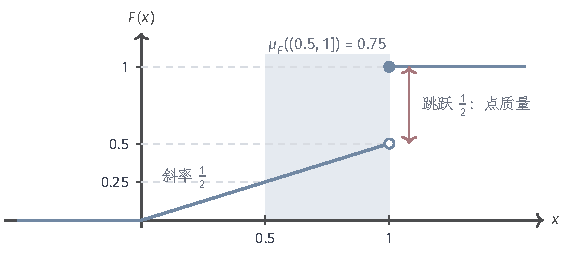
\includegraphics[width=96.5mm]{figures/02-abstract-mathematics/01-metric-and-measure/tikz/c2-stieltjes-jump/figure.pdf}
  \caption{右连续单调函数$F$确定的Lebesgue--Stieltjes测度。$F$在$[0,1)$上以斜率$1/2$增长，对应总量$1/2$、均匀分布在$[0,1]$上的质量；在$x=1$处跳跃$1/2$（实心点为$F(1)=1$，空心点为左极限$1/2$），对应点质量$\tfrac12\delta_1$。阴影竖条示意区间$(0.5,1]$的测度$F(1)-F(0.5)=0.75$。}
  \label{fig:measure-stieltjes-jump}
\end{figure}

连续的$F$不产生点质量，但这不意味着$\mu_F$一定像长度那样“摊开”分布。第~\ref{sec:measure-decomposition}节将用Cantor集构造一个连续的$F$，它的测度集中在零测的Cantor集上；至于$\mu_F$何时能表示成相对于长度的密度，留到第~\ref{chap:densities-change-of-measure}章回答。
